\documentclass[a4paper, 10pt]{book}

\usepackage{tcolorbox}

\usepackage{wrapfig}

\usepackage{graphicx}
\usepackage{float}

\usepackage{tikz}
\usepackage{amsmath}
\usepackage{forest}
\usetikzlibrary{shadows}


\usepackage{fontspec} % --fontspec-- package to use other fonts
\setmainfont{Vazirmatn-Regular.ttf} 
\newfontfamily\bold{Vazirmatn-Bold.ttf}

\usepackage{hyperref}

\usepackage{color}

\usepackage{geometry}
\geometry{top=2cm, bottom=2cm, left=1.5cm, right=1.5cm}

\title{\huge {\bold Parallel Algorithms}}
\author{Professor\\{\bold Dr. Masoumeh Damroudi}}
\date{Author\\{\bold Mohammad Khorshidi}}

\linespread{1.3}

\begin{document}

    \pagenumbering{roman}
    \maketitle
    \newpage

    \begin{center}
        \Large {\bold Course Overview}
    \end{center}

    In this lecture note, I have documented my personal interpretations and understanding of the material. Please note that there may be inaccuracies, and it is recommended to consult primary and authoritative sources for complete and accurate information. Additionally, I welcome any contributions to improve and refine this note. If you are reading this and would like to offer suggestions, feel free to do so via pull requests on my \href{https://github.com/elprofesorsunny/Master/tree/main/Papers/Parallel%20Aalgorithms/Booklet}{\textcolor{blue}{\bold GitHub}} or by emailing me at \href{mailto:someone@somewhere.com}{\textcolor{blue}{\bold mohammad\_khorshidi@outlook.fr}}.

    \section{Course Structure}

    \section{Instructor's Approach}

    \section{Grading and Evaluation}

        The grading structure for this course is as follows, with students expected to earn their grades based on the criteria outlined below:

        \begin{itemize}
            
            \item {\bold Presentation:} 4 points will be awarded for presenting and explaining a paper related to one aspect of parallelization, accompanied by its relevant implementation.

            \item {\bold Midterm Exam:} 4 points will be given for the midterm exam.

            \item {\bold Final Exam:} 12 points will be awarded for the final exam.

        \end{itemize}

        Additionally, students are expected to attend all classes and give due attention to the assignments that will be provided throughout the semester.
        
    \section{Course Materials and Resources}

    \tableofcontents
    
    \chapter{{\bold Introduction}}

    \pagenumbering{arabic}

        In today’s world, with the increasing volume of data and the need for faster computations, parallel algorithms have emerged as an effective method to enhance the performance of computing systems. Parallel algorithms allow us to divide a problem into smaller sub-problems, each of which can be processed simultaneously by multiple processors. This not only speeds up processing but also optimizes the use of hardware resources.

        In this lecture note, we will explore fundamental concepts of parallel processing, computational models such as the PRAM model, and interconnection structures like network links. We will also delve into the principles of designing and analyzing parallel algorithms, covering key metrics such as performance, speedup, and scalability. Our goal is to provide a comprehensive understanding of the challenges and opportunities in the field of parallel algorithms.

        Parallel algorithms play a crucial role in improving the performance of complex and resource-intensive computations. The primary goal of parallel algorithms is to divide a large problem into smaller, independent sub-problems, which can be solved simultaneously by multiple processors. This technique is essential in multi-core and distributed computing environments such as supercomputers and large computing clusters.

        The need for parallel computation arises from the requirement to process large amounts of data or perform complex computations in a reasonable amount of time. A parallel computer, which consists of multiple processing units or processors, enables this by dividing a large problem into smaller sub-problems. Each of these sub-problems is solved independently and simultaneously by separate processors. The results are then combined to solve the original problem more efficiently.

        This approach, known as parallel computing, leverages the power of multiple processors to work on different parts of a problem at the same time. By doing so, it accelerates the overall computation and makes optimal use of hardware resources. Algorithms that are specifically designed to utilize parallel computing, called parallel algorithms, are key to solving complex problems faster and more efficiently by running them on parallel computer architectures.

        \section{Computational Models}

            In any computing system, whether sequential or parallel, the instructions are executed based on the flow of data. The execution flow dictates the sequence in which the tasks are carried out by the computer and what needs to be done at each stage of execution.

            The flow of data through the instructions influences how they operate. Understanding the correct computational model is crucial for designing parallel algorithms. These models determine the architecture and behavior of the system, impacting the performance and efficiency of parallel computation.

            Flynn, in 1966, introduced a taxonomy of computer architectures based on instruction and data streams. The four major classes of this classification are:

            \begin{itemize}
                
                \item {\bold SISD (Single Instruction, Single Data):} A single instruction is executed on a single data stream.
                
                \item {\bold MISD (Multiple Instruction, Single Data):} Multiple instructions are executed on a single data stream.

                \item {\bold SIMD (Single Instruction, Multiple Data):} A single instruction is executed on multiple data streams simultaneously.

                \item {\bold MIMD (Multiple Instruction, Multiple Data):} Multiple instructions are executed on multiple data streams simultaneously.

            \end{itemize}

            \begin{figure}[H]

                \centering
                
                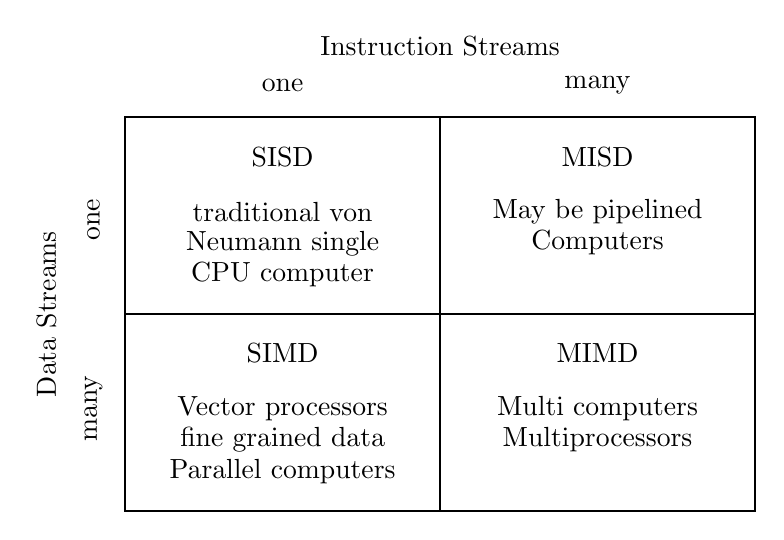
\begin{tikzpicture}
                    % Draw the grid lines
                    \draw[thick] (0,0) rectangle (8,5);
                    \draw[thick] (0,2.5) -- (8,2.5);
                    \draw[thick] (4,0) -- (4,5);
                    
                    % Add labels for SISD, SIMD, MISD, MIMD
                    \node at (2,4.5) {{\bold SISD}};
                    \node at (6,4.5) {{\bold MISD}};
                    \node at (2,2) {{\bold SIMD}};
                    \node at (6,2) {{\bold MIMD}};
                    
                    % Add descriptions for each category
                    \node at (2,3.8) {traditional von};
                    \node at (2,3.4) {Neumann single};
                    \node at (2,3) {CPU computer};
                    
                    \node at (6,3.8) {May be pipelined};
                    \node at (6,3.4) {Computers};
                    
                    \node at (2,1.3) {Vector processors};
                    \node at (2,0.9) {fine grained data};
                    \node at (2,0.5) {Parallel computers};
                    
                    \node at (6,1.3) {Multi computers};
                    \node at (6,0.9) {Multiprocessors};
                    
                    % Label axes
                    \node[rotate=90] at (-1,2.5) {Data Streams};
                    \node[rotate=90] at (-0.4,3.7) {one};
                    \node[rotate=90] at (-0.4,1.3) {many};
                    
                    \node at (2,5.4) {one};
                    \node at (6,5.4) {many};
                    \node at (4,5.9) {Instruction Streams};
                    
                \end{tikzpicture}
                
                \caption{A comparison between SISD, MISD, SIMD, and MIMD architectures}
            
            \end{figure}

            \subsection{SISD Architecture}

                \begin{wrapfigure}{r}{0.5\textwidth}

                    \centering

                    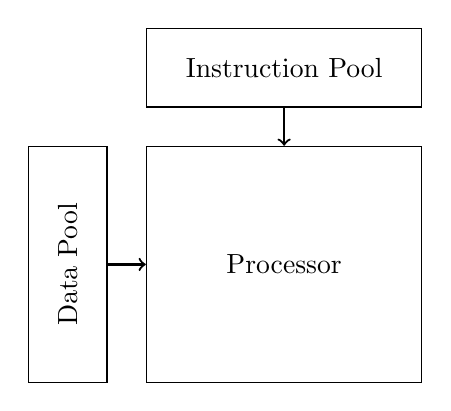
\begin{tikzpicture}

                            % Data Pool
                            \node[draw, minimum width=3cm, minimum height=1cm, rotate=90]  (data) at (0.25,0) {Data Pool};

                            % Instruction Pool
                            \node[draw, minimum width=3.5cm, minimum height=1cm] (instruction) at (3,2.5) {Instruction Pool};

                            % Processor
                            \node[draw, minimum width=3.5cm, minimum height=3cm] (processor) at (3,0) {{\bold Processor}};

                            % Arrows
                            \draw[thick, ->] (data.south) -- (processor.west);
                            \draw[thick, ->] (instruction.south) -- (processor.north);

                    \end{tikzpicture}

                    \caption{A conceptual diagram of SISD architecture.}

                \end{wrapfigure}

                The Single Instruction Single Data (SISD) architecture, introduced by John von Neumann in the late 1940s, processes one instruction at a time over a single data stream. This sequential nature means it doesn't support parallel processing, requiring only one processor to execute the tasks.

                An SISD computing system is a uniprocessor machine which is capable of executing a single instruction, operating on a single data stream. In SISD, machine instructions are processed in a sequential manner and computers adopting this model are popularly called sequential computers. Most conventional computers have SISD architecture. All the instructions and data to be processed have to be stored in primary memory.

                In the SISD model, the algorithm works in a serial fashion. For example, to sum a sequence of $n$ numbers, the algorithm accesses the memory $n$ times and performs $n−1$ additions. The time complexity for this approach can be expressed as:
        
                $$O(n)$$

                Where:

                \begin{itemize}
                    
                    \item $n$: The number of elements to process.

                    \item $O(n)$: Reflects that the algorithm's running time scales linearly with the size of the input.

                \end{itemize}

                In this architecture, there is no room for parallelism, and each operation occurs sequentially, requiring every data element to be processed one at a time. For a sum operation on $n$ numbers:

                \begin{itemize}

                    \item Memory accesses: $n$ memory fetches.
                    \item Additions: $n−1$ addition operations.

                \end{itemize}

                Thus, the total computational complexity is linear, i.e., $O(n)$, representing the number of accesses and operations required to complete the task. For this type of architecture, the performance is highly dependent on the efficiency of the processor and memory access speed, as there is no way to split the workload across multiple processors.
                
            \subsection{MISD Architecture}

                \begin{wrapfigure}{r}{0.5\textwidth}
                
                \centering
                
                    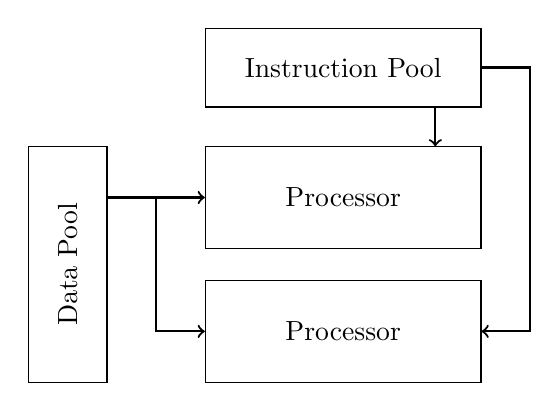
\begin{tikzpicture}

                            % Data Pool
                            \node[draw, minimum width=3cm, minimum height=1cm, rotate=90]  (data) at (-0.5,0) {Data Pool};

                            % Instruction Pool
                            \node[draw, minimum width=3.5cm, minimum height=1cm] (instruction) at (3,2.5) {Instruction Pool};

                            % Processors
                            \node[draw, minimum width=3.5cm, minimum height=1.3cm] (processor1) at (3,0.85) {{\bold Processor}};
                            \node[draw, minimum width=3.5cm, minimum height=1.3cm] (processor2) at (3,-0.85) {{\bold Processor}};

                            % Arrows
                            % Arrow from Data Pool to junction point
                            \draw[thick, ->] (0,0.85) -- (processor1.west);

                            % Arrow from junction point to Processor2
                            \draw[thick, ->] (0.625, 0.85) -- (0.625, -0.85) -- (processor2.west);

                            % Arrow from Instruction Pool to Processor1 (straight)
                            \draw[thick, ->] (4.17,2) -- (4.17,1.5);

                            % Arrow from Instruction Pool to Processor2 (broken path)
                            \draw[thick, ->] (instruction.east) -- (5.375, 2.5) -- (5.375, -0.85) -- (processor2.east);

                    \end{tikzpicture}

                    \caption{A conceptual diagram of MISD architecture.}

                \end{wrapfigure}

                The Multiple Instruction Single Data (MISD) is a less common architecture where multiple processors execute different instructions but operate on the same data stream simultaneously. This approach is primarily used in specialized applications like fault-tolerant systems or systems requiring redundancy. The MISD model is structured to handle cases where having multiple processors work on the same data but with different operations is crucial.

                In MISD architecture, each processor has its own control unit that dictates the operations performed. Unlike SIMD, which focuses on parallel data processing, MISD involves parallel instruction execution on a single data stream. To illustrate, imagine a real-time safety system where different sensors provide data that multiple processors analyze for distinct purposes:

                \begin{itemize}
                    
                    \item {\bold Processor 1} checks if the temperature is within a safe range.
                
                    \item {\bold Processor 2} monitors the pressure of the system.

                    \item {\bold Processor 3} assesses voltage levels.

                \end{itemize}

                All processors work on the same data stream from the sensors but perform different tasks to ensure system reliability and fault tolerance. If any processor detects a problem, the system can react accordingly to prevent failure.

                In a typical MISD system:

                \begin{itemize}

                    \item Multiple processors (N) receive the same input data simultaneously.

                    \item Each processor is responsible for executing a unique instruction on that shared data stream.

                    \item The processors operate in parallel, but the parallelism applies to the instruction execution, not to the data.

                \end{itemize}

                This kind of architecture is rare due to its niche applicability, often used in scenarios where redundancy is crucial, such as avionics or control systems, where the same data needs to be processed in multiple ways to ensure accuracy and safety.

                The time complexity of an MISD system depends heavily on the operations performed by each processor. Each processor runs independently, and the overall time to process the data is determined by the slowest processor, similar to SISD's sequential operation but distributed across different instruction sets.

                For N processors with execution times $T_1, T_2, \dots, T_N$, the overall time complexity is governed by the maximum time:

                $$T_{total}=max(T_1, T_2, \dots, T_N)$$

                This means the overall system performance is constrained by the processor taking the longest to complete its task.

            \subsection{SIMD Architecture}

                The Single Instruction Multiple Data (SIMD) architecture enables a single instruction to operate simultaneously across multiple data streams. In this model, one instruction, such as an addition or comparison, is applied to different sets of data in parallel, which significantly enhances processing efficiency.

                In an SIMD system, there are N identical processors, all controlled by a single stream of instructions from a central control unit. Each processor executes the same instruction but operates on its own separate data stream. Therefore, N data streams exist, with one data stream assigned to each processor.

                Communication between processors for data transfer in SIMD computers can occur in two main ways:

                \begin{enumerate}
                    
                    \item {\bold Shared memory:} All processors access a common memory space to fetch or store data.

                    \item {\bold Interconnection networks:} A specialized network connects the processors to facilitate data transfer between them.

                \end{enumerate}

                SIMD architecture is particularly well-suited for tasks requiring parallel data processing, such as graphical computations or heavy workloads where operations need to be performed on multiple data elements simultaneously. For example, in image or video processing, SIMD can process multiple pixels or image sections in parallel, leading to a significant speedup in computation.

                \subsubsection{{\bold > \hspace{10pt} Shared Memory (SM) SIMD Computers}}

                    In Shared-Memory (SM) SIMD computers, the communication between processors occurs through a shared memory space. This model is often referred to as the Parallel Random-Access Machine (PRAM) model, where multiple processors work in parallel, and data exchange happens via common memory access.

                    When a processor (say {\bold processor i}) wants to send data to another processor ({\bold processor j}), the process follows two key steps:

                    \begin{enumerate}
                        
                        \item {\bold Processor i} writes the data into a known location in the shared memory, which {\bold processor j} can access.

                        \item {\bold Processor j} then reads the data from that specific location.
                        
                    \end{enumerate}

                    SIMD shared-memory computers are categorized based on how processors can concurrently access the same memory location. These categories determine how simultaneous read and write operations are handled, as follows:

                    \begin{itemize}
                        
                        \item {\bold Exclusive-Read, Exclusive-Write (EREW):} No two processors can read from or write to the same memory location at the same time.

                        \item {\bold Concurrent-Read, Exclusive-Write (CREW):} Multiple processors can read from the same memory location simultaneously, but only one can write to a memory location at any given time.

                        \item {\bold Exclusive-Read, Concurrent-Write (ERCW):} Only one processor can read from a memory location at a time, but multiple processors can write to the same location simultaneously.

                        \item {\bold Concurrent-Read, Concurrent-Write (CRCW):} Both read and write operations can be performed by multiple processors on the same memory location simultaneously.

                    \end{itemize}
                
                    These categories define the degree of parallelism and the restrictions on data sharing among processors in a shared-memory SIMD system.

                    \begin{tcolorbox}[colback=white, colframe=black!25, title=Example]
                    
                        Searching for element x in an unordered file with n distinct entries using different SIMD models.
    
                        \begin{minipage}{0.49\linewidth} % First
                            \footnotesize
                            \vspace{0.3cm}
                            \begin{tcolorbox}[colframe=white, size=small]
    
                                {\bold Using the EREW Model with N processors where $N\geq n$}
                                
                                \vspace{0.3cm}

                                {\bold Phase 1:}
                                
                                Broadcasting the value of x to all processors in  $O(N\log N)$ time
    
                                \begin{itemize}
                                    
                                    \item Processor P1 sends x to P3 and P2 sends x to P4, and so on.
                                    \item This process continues until all processors have the value x.
    
                                \end{itemize}
    
                                {\bold Phase 2:}
                                
                                Simultaneous search in sub-files by processors in $O(\frac{N}{n})$ time.
                                
                                \begin{itemize}
                                    
                                    \item Processor P1 searches the first $\frac{n}{N}$ data.
                                    \item Processor P2 searches the second $\frac{n}{N}$ data.
                                    \item And so on for all N processors.
    
                                \end{itemize}
    
                                Initially, F is set to false. The first processor to find x sets F to true. All processors check F at each step, and if F becomes true, the search ends. The broadcast of F takes $O(\log N)$ time per step.
                                In the worst case, the EREW model requires $+ O(N\log N(N \log(\frac{N}{n})))$ time.
                            \end{tcolorbox}
                        \end{minipage}
                        \hfill
                        \begin{minipage}{0.49\linewidth} % Second
                            \footnotesize
                            \vspace{0.3cm}
                            \begin{tcolorbox}[colframe=white, size=small]
    
                                {\bold Using the CREW Model with N processors where $N\geq n$}
    
                                \vspace{0.3cm}

                                {\bold Phase 1:}
                                
                                Broadcasting the value of x to all processors in parallel using a single write per memory location.
    
                                \begin{itemize}
                                    
                                    \item Since concurrent reads are allowed, all processors can read the value of x from a shared memory location at the same time, significantly speeding up the process.
    
                                    \item This reduces the broadcast time to $O(\log N)$ since only one write operation is needed.
    
                                \end{itemize}

                                {\bold Phase 2:}
                                
                                Simultaneous search in sub-files by processors in $O(\frac{N}{n})$ time.
    
                                \begin{itemize}
                                    
                                    \item Similar to the EREW model, P1 searches the first $\frac{n}{N}$ data, P2 searches the second, and so on.
    
                                    \item As soon as one processor finds x, it updates F to true, and the search ends.
    
                                \end{itemize}
    
                                With concurrent reads, the worst-case time complexity is reduced to $N\log (\frac{N}{n})+O(\log N)$.
    
                            \end{tcolorbox}
                        \end{minipage}
    
                        \begin{minipage}{0.49\linewidth} % Thired
                            \footnotesize
                            \vspace{0.3cm}
                            \begin{tcolorbox}[colframe=white, size=small]
    
                                {\bold Using the ERCW Model with N processors where $N\geq n$}
    
                                \vspace{0.3cm}

                                {\bold Phase 1:}
                                
                                Broadcasting x to all processors in $O(\log N)$ time.
    
                                \begin{itemize}
                                    
                                    \item Similar to CREW, all processors can read x from a shared location.
    
                                \end{itemize}
    
                                {\bold Phase 2:}
                                
                                Simultaneous search in sub-files by processors in $O(\frac{N}{n})$ time.
    
                                \begin{itemize}
                                    
                                    \item Again, processors search different parts of the data in parallel.
                                    
                                    \item However, here multiple processors can concurrently write to the same memory location. If one processor finds x, it writes to the shared F location. Other processors can also attempt to write, but only one write will succeed.
    
                                \end{itemize}
    
                                With concurrent writes, the time complexity remains $+O(\log N(N \log(\frac{N}{n})))$, though write conflicts may slightly impact performance.
    
                            \end{tcolorbox}
                        \end{minipage}
                        \hfill
                        \begin{minipage}{0.49\linewidth} % Fourth
                            \footnotesize
                            \vspace{0.3cm}
                            \begin{tcolorbox}[colframe=white, size=small]
                                
                                {\bold Using the CRCW Model with N processors where $N\geq n$}
    
                                {\bold Phase 1:}
                                
                                Broadcasting x to all processors in constant time $O(1)$.
    
                                \begin{itemize}
                                    
                                    \item In this model, both reads and writes are performed concurrently, so all processors can obtain the value of x simultaneously from the shared memory.
    
                                \end{itemize}
    
                                {\bold Phase 2:}
                                
                                Simultaneous search in sub-files by processors in parallel.
    
                                \begin{itemize}
                                    
                                    \item Each processor searches its assigned portion of the data. Once a processor finds x, it writes true to F, and the search concludes. Since multiple writes are allowed at the same memory location, any processor finding x can update F without delay.
    
                                \end{itemize}
                                
                                The worst-case time complexity for CRCW is minimized to $O(\frac{N}{n})$ because concurrent reading and writing reduce the overhead. 
                            
                            \end{tcolorbox}
                        \end{minipage}
                    
                    \end{tcolorbox}

                    When designing shared-memory SIMD computers, one of the main challenges is how to efficiently manage access to memory locations shared by multiple processors. The key concern is the cost of routing data between processors and memory, which scales with the number of processors $N$ and memory locations $M$. Now the problem overview raised is below:

                    \begin{itemize}
                        
                        \item Memory circuits need to be established to create pathways between the processors and the shared memory locations.

                        \item If each processor has its own dedicated memory, the cost for this approach is proportional to $f(M)$.

                        \item Sharing memory among processors reduces the total memory cost, but for large $N$ and $M$, the circuit cost can still become significant, growing proportionally to $N \times f(M)$.

                    \end{itemize}

                    To address this problem, several strategies have been proposed:

                    \begin{enumerate}
                        
                        \item {\bold Approach 1:} Dividing shared memory into $R$ blocks of equal size, where each processor can access a block of memory at a time ($\frac{M}{R}$). This reduces the required memory per processor.

                        \item {\bold Approach 2:} Distributing $N$ memory locations equally among $N$ processors, with each processor handling a specific portion of the memory ($\frac{M}{N}$). This helps balance the workload and reduce memory contention.

                    \end{enumerate}

                    \begin{tcolorbox}[colback=white, colframe=black!25, title= Example$:$ Memory Partitioning and Access (SM SIMD)]
                    
                        In more detail, consider the scenario where memory is shared between $N$ processors by dividing the memory into $R$ blocks of equal size, where each processor can access one block at a time. For example, if $R = 3$ and $N = 5$, the processors share memory with each accessing its respective block.

                        \begin{minipage}{0.49\linewidth}
                            \footnotesize
                            \vspace{0.3cm}
                            \begin{tcolorbox}[colframe=white, size=small]
                                
                                {\bold Key Points:}

                                \begin{itemize}
                                    
                                    \item In each time step, a processor can only access one block of shared memory ($\frac{M}{R}$).

                                    \item The $N + R$ bidirectional links provide access between each processor and its designated block of memory.

                                    \item The overall circuit cost grows according to $N \times R \times f(\frac{M}{R})$, with an additional switch needed for managing simultaneous access.

                                \end{itemize}
                                
                            \end{tcolorbox}
                        \end{minipage}
                        \hfill
                        \begin{minipage}{0.49\linewidth}
                            \footnotesize
                            \vspace{0.3cm}
                            \begin{tcolorbox}[colframe=white, size=small]
                                
                                In practice, this model ensures efficient memory access without overwhelming the system with excessive memory demands, but it requires careful management of access timing and switching to avoid conflicts.

                            \end{tcolorbox}
                        \end{minipage}

                        \vspace{0.4cm}
                        \begin{center}
                            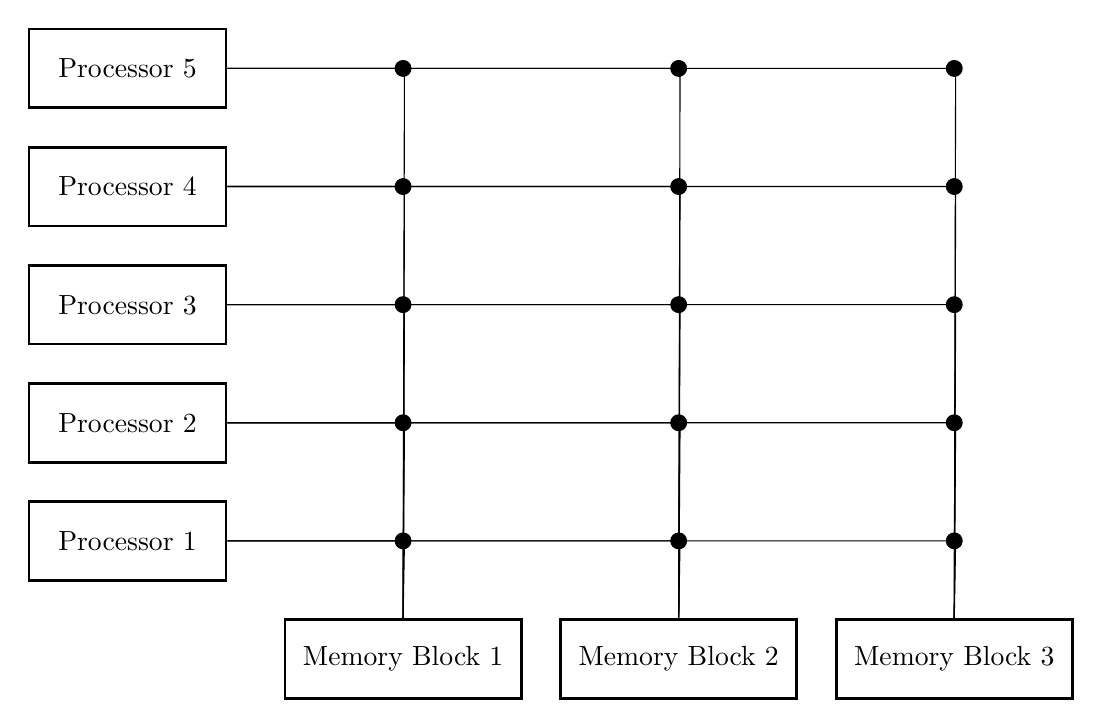
\begin{tikzpicture}
                                
                                % Processors
                                \node[draw, minimum width=2.5cm, minimum height=1cm, line width=1] (P1) at (0,0) {\bold Processor 1};
                                \node[draw, minimum width=2.5cm, minimum height=1cm, line width=1] (P2) at (0,1.5) {\bold Processor 2};
                                \node[draw, minimum width=2.5cm, minimum height=1cm, line width=1] (P3) at (0,3) {\bold Processor 3};
                                \node[draw, minimum width=2.5cm, minimum height=1cm, line width=1] (P4) at (0,4.5) {\bold Processor 4};
                                \node[draw, minimum width=2.5cm, minimum height=1cm, line width=1] (P5) at (0,6) {\bold Processor 5};
                                
                                % Memories
                                \node[draw, minimum width=3cm, minimum height=1cm, line width=1] (M1) at (3.5,-1.5) {\bold Memory Block 1};
                                \node[draw, minimum width=3cm, minimum height=1cm, line width=1] (M2) at (7,-1.5) {\bold Memory Block 2};
                                \node[draw, minimum width=3cm, minimum height=1cm, line width=1] (M3) at (10.5,-1.5) {\bold Memory Block 3};

                                % Joints
                                \foreach \i in {1,2,3,4,5} {
                                    \foreach \j in {1} {
                                        \draw[-] (P\i.east) -- ++(2.25,0) -- (M\j.north);
                                        }
                                        }
                                
                                \foreach \i in {1,2,3,4,5} {
                                    \foreach \j in {2} {
                                        \draw[-] (P\i.east) -- ++(5.75,0) -- (M\j.north);
                                        }
                                        }

                                \foreach \i in {1,2,3,4,5} {
                                    \foreach \j in {3} {
                                        \draw[-] (P\i.east) -- ++(9.25,0) -- (M\j.north);
                                        }
                                        }

                                % Circles
                                \draw[black, fill=black] (3.5,0) circle (0.1cm);
                                \draw[black, fill=black] (7,0) circle (0.1cm);
                                \draw[black, fill=black] (10.5,0) circle (0.1cm);
                                \draw[black, fill=black] (3.5,1.5) circle (0.1cm);
                                \draw[black, fill=black] (7,1.5) circle (0.1cm);
                                \draw[black, fill=black] (10.5,1.5) circle (0.1cm);
                                \draw[black, fill=black] (3.5,3) circle (0.1cm);
                                \draw[black, fill=black] (7,3) circle (0.1cm);
                                \draw[black, fill=black] (10.5,3) circle (0.1cm);
                                \draw[black, fill=black] (3.5,4.5) circle (0.1cm);
                                \draw[black, fill=black] (7,4.5) circle (0.1cm);
                                \draw[black, fill=black] (10.5,4.5) circle (0.1cm);
                                \draw[black, fill=black] (3.5,6) circle (0.1cm);
                                \draw[black, fill=black] (7,6) circle (0.1cm);
                                \draw[black, fill=black] (10.5,6) circle (0.1cm);
                                    
                            \end{tikzpicture}
                        \end{center}
                        \vspace{0.4cm}

                    \end{tcolorbox}

                \subsubsection{{\bold > \hspace{10pt} Interconnection Network (IN) SIMD Computers}}

                    In SIMD computers, interconnection networks play a crucial role in efficiently distributing and processing data across multiple processors. The memory is distributed evenly between $N$ processors, and each processor is connected to others, facilitating data exchange. In fully connected networks, every processor is directly connected to every other processor, ensuring fast communication and reducing latency. The communication cost, however, increases significantly as the number of processors grows, following the relationship $O(N^2)$ for connection setup.

                    Interconnection networks can be classified into two main types:

                    \begin{itemize}
                        
                        \item {\bold Dynamic Networks:} The connections are configured dynamically, adjusting based on the specific task or algorithm.

                        \item {\bold Static Networks:} These networks have fixed, unchanging connections between processors.

                    \end{itemize}

                    Dynamic and static networks can further be differentiated based on their topologies. Topologies are the physical or logical arrangement of the network, defining how processors are interconnected. For SIMD computers, static networks are more common due to their simplicity and ease of design, and they include structures like linear arrays, trees, rings, and hypercubes. Each topology offers a different balance between complexity, cost, and communication speed, impacting the overall performance of the system. Compared to models like MISD, static interconnection networks in SIMD computers are easier to design, and the underlying algorithms are simpler. These systems are most suited for problems where data is evenly distributed among processors and need to be processed concurrently.

                    When designing interconnection networks, key factors include:

                    \begin{itemize}
                        
                        \item {\bold Degree:} The maximum number of direct connections a processor can have.

                        \item {\bold Diameter:} The longest distance between any two processors in the network.

                        \item {\bold Bisection Width:} The minimum number of connections that must be removed to split the network into two equal halves.

                    \end{itemize}

                    Different topologies offer varying levels of performance based on these parameters. For instance, a completely connected network provides the best communication speed, but at the cost of increased complexity in wiring and connection management.

                    \begin{center}
                        
                        \begin{forest}
                            for tree={rounded corners,
                            draw,
                            text centered,
                            anchor=north,
                            grow=east,
                            anchor=west,
                            parent anchor=east,
                            child anchor=west,
                            l sep=1cm,
                            s sep=0.2cm,
                            tier/.wrap pgfmath arg={level#1}{level()}
                            }
                            [Static Interconnection Networks
                                [LCN
                                    [Hybrid
                                        [Pyramid]
                                        [Diamond]
                                        [MMT]
                                    ]
                                    [4D
                                        [Hypercube]
                                    ]
                                    [3D
                                        [3D Mesh]
                                        [Cube]
                                    ]
                                    [2D
                                        [Ring]
                                        [Mesh]
                                        [2D Torus]
                                        [ILLIAC]
                                        [Fat Tree]
                                        [Tree]
                                    ]
                                    [1D
                                        [Linear Array]
                                    ]
                                ]
                                [CCN
                                    [Completely Connected]
                                ]
                            ]
                        \end{forest}
                    \end{center}

                    Here's a detailed overview of the various static interconnection network topologies depicted in the diagram. These topologies represent different ways to connect processors and memory blocks in parallel computing systems, ensuring efficient communication between different processing elements (PEs). Each topology has its own unique structure, offering distinct advantages in terms of latency, scalability, and fault tolerance. The choice of an appropriate interconnection network plays a crucial role in optimizing the performance of SIMD or MIMD systems, depending on the specific requirements of the task at hand.

                    \vspace{0.4cm}
                    \noindent
                    \begin{minipage}{0.49\linewidth} % Linear Array
                        \begin{tcolorbox}[colframe=black!50, colback=white, size=small]

                            {\bold Linear Array}
                            
                            Processors are connected in a straight line, with each processor linked to its immediate neighbor.

                            \begin{center}
                                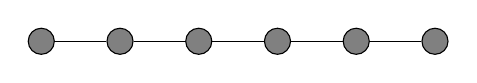
\begin{tikzpicture}
                                    
                                    \foreach \i in {1,...,6}
                                        \node[circle, draw, fill=black!50] (n\i) at (\i,0) {};

                                    \foreach \i in {1,...,5}
                                        \draw (n\i) -- (n\the\numexpr\i+1);

                                \end{tikzpicture}
                            \end{center}

                        \end{tcolorbox}
                    \end{minipage}
                    \hfill
                    \begin{minipage}{0.49\linewidth}
                        \begin{tcolorbox}[colframe=black!50, colback=white, size=small]
                            
                            {\bold Mesh}
                            
                            Processors are arranged in a 2D grid, with each processor connected to its four adjacent neighbors.

                            \begin{center}
                                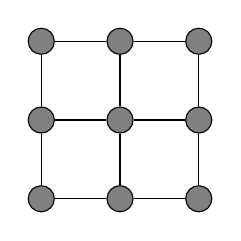
\begin{tikzpicture}
                                    
                                    \foreach \x in {1,2,3}
                                        \foreach \y in {1,2,3}
                                            \node[circle, draw, fill=black!50] (n\x\y) at (\x, \y) {};
                                
                                    \foreach \x in {1,2}
                                        \foreach \y in {1,2,3}
                                            \draw (n\x\y) -- (n\the\numexpr\x+1 \y);
                                    
                                    \foreach \x in {1,2,3}
                                        \foreach \y in {1,2}
                                            \draw (n\x\y) -- (n\x\the\numexpr\y+1);

                                \end{tikzpicture}
                            \end{center}

                        \end{tcolorbox}                        
                    \end{minipage}

                    \vspace{0.3cm}
                    \noindent
                    \begin{minipage}{0.49\linewidth}
                        \begin{tcolorbox}[colframe=black!50, colback=white, size=small]
                            
                            {\bold Tree}
                            
                            A hierarchical structure where each node (processor) has a parent-child relationship, used for efficient data propagation.

                            \begin{center}
                                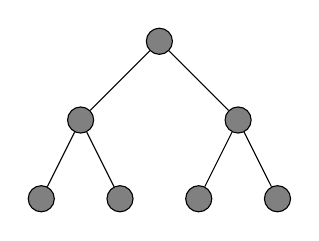
\begin{tikzpicture}
                                    
                                    \node[circle, draw, fill=black!50] (root) at (0,2) {};
    
                                    \node[circle, draw, fill=black!50] (n1) at (-1,1) {};
                                    \node[circle, draw, fill=black!50] (n2) at (1,1) {};
                                    
                                    \node[circle, draw, fill=black!50] (n3) at (-1.5,0) {};
                                    \node[circle, draw, fill=black!50] (n4) at (-0.5,0) {};
                                    \node[circle, draw, fill=black!50] (n5) at (0.5,0) {};
                                    \node[circle, draw, fill=black!50] (n6) at (1.5,0) {};
                                    
                                    \draw (root) -- (n1);
                                    \draw (root) -- (n2);
                                    \draw (n1) -- (n3);
                                    \draw (n1) -- (n4);
                                    \draw (n2) -- (n5);
                                    \draw (n2) -- (n6);

                                \end{tikzpicture}
                            \end{center}

                        \end{tcolorbox}
                    \end{minipage}
                    \hfill
                    \begin{minipage}{0.49\linewidth}
                        \begin{tcolorbox}[colframe=black!50, colback=white, size=small]

                            {\bold Hypercube}
                            
                            An extension of the cube structure with more dimensions, providing even faster communication and better fault tolerance.

                            \begin{center}
                                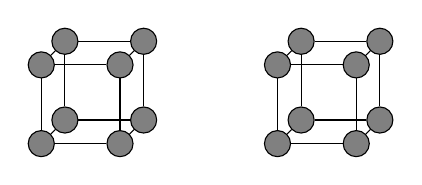
\begin{tikzpicture}

                                    \node[circle, draw, fill=black!50] (n1) at (0,0) {};
                                    \node[circle, draw, fill=black!50] (n2) at (0,1) {};
                                    \node[circle, draw, fill=black!50] (n3) at (1,0) {};
                                    \node[circle, draw, fill=black!50] (n4) at (1,1) {};

                                    \node[circle, draw, fill=black!50] (n5) at (0.3,0.3) {};
                                    \node[circle, draw, fill=black!50] (n6) at (0.3,1.3) {};
                                    \node[circle, draw, fill=black!50] (n7) at (1.3,0.3) {};
                                    \node[circle, draw, fill=black!50] (n8) at (1.3,1.3) {};

                                    \node[circle, draw, fill=black!50] (n9) at (3,0) {};
                                    \node[circle, draw, fill=black!50] (n10) at (3,1) {};
                                    \node[circle, draw, fill=black!50] (n11) at (4,0) {};
                                    \node[circle, draw, fill=black!50] (n12) at (4,1) {};
                                    
                                    \node[circle, draw, fill=black!50] (n13) at (3.3,0.3) {};
                                    \node[circle, draw, fill=black!50] (n14) at (3.3,1.3) {};
                                    \node[circle, draw, fill=black!50] (n15) at (4.3,0.3) {};
                                    \node[circle, draw, fill=black!50] (n16) at (4.3,1.3) {};

                                    \draw (n1) -- (n2);
                                    \draw (n1) -- (n3);
                                    \draw (n1) -- (n5);
                                    \draw (n2) -- (n4);
                                    \draw (n2) -- (n6);
                                    \draw (n3) -- (n4);
                                    \draw (n3) -- (n7);
                                    \draw (n4) -- (n8);
                                    \draw (n5) -- (n6);
                                    \draw (n5) -- (n7);
                                    \draw (n6) -- (n8);
                                    \draw (n7) -- (n8);
                                    
                                    \draw (n9) -- (n10);
                                    \draw (n9) -- (n11);
                                    \draw (n9) -- (n13);
                                    \draw (n10) -- (n12);
                                    \draw (n10) -- (n14);
                                    \draw (n11) -- (n12);
                                    \draw (n11) -- (n15);
                                    \draw (n12) -- (n16);
                                    \draw (n13) -- (n14);
                                    \draw (n13) -- (n15);
                                    \draw (n14) -- (n16);
                                    \draw (n15) -- (n16);

                                    
                                \end{tikzpicture}
                            \end{center}

                        \end{tcolorbox}
                    \end{minipage}
                    
                    \vspace{0.3cm}
                    \noindent
                    \begin{minipage}{0.49\linewidth}
                        \begin{tcolorbox}[colframe=black!50, colback=white, size=small]
                            
                            {\bold Cube}
                            
                            Processors are connected in the shape of a 3D cube, offering fast communication between nearby nodes.

                            \begin{center}
                                \begin{tikzpicture}

                                    
                                    
                                \end{tikzpicture}
                            \end{center}

                        \end{tcolorbox}
                    \end{minipage}
                    \hfill
                    \begin{minipage}{0.49\linewidth}
                        \begin{tcolorbox}[colframe=black!50, colback=white, size=small]
                            
                            {\bold Ring}
                            
                            Processors form a circular connection where each one is linked to two neighbors, forming a loop.

                            \begin{center}
                                \begin{tikzpicture}

                                    
                                    
                                \end{tikzpicture}
                            \end{center}

                        \end{tcolorbox}
                    \end{minipage}
                    
                    \vspace{0.3cm}
                    \noindent
                    \begin{minipage}{0.49\linewidth}
                        \begin{tcolorbox}[colframe=black!50, colback=white, size=small]

                            {\bold Completely Connected}
                            
                            Every processor is directly connected to every other processor, allowing the fastest possible communication.

                            \begin{center}
                                \begin{tikzpicture}

                                    
                                    
                                \end{tikzpicture}
                            \end{center}

                        \end{tcolorbox}
                    \end{minipage}
                    \hfill
                    \begin{minipage}{0.49\linewidth}
                        \begin{tcolorbox}[colframe=black!50, colback=white, size=small]
                            
                            {\bold Fat Tree}
                            
                            A tree structure with more bandwidth at higher levels, commonly used for network switches to balance loads.

                            \begin{center}
                                \begin{tikzpicture}

                                    
                                    
                                \end{tikzpicture}
                            \end{center}
                            
                        \end{tcolorbox}
                    \end{minipage}
                    
                    \vspace{0.3cm}
                    \noindent
                    \begin{minipage}{0.49\linewidth}
                        \begin{tcolorbox}[colframe=black!50, colback=white, size=small]
                            
                            {\bold ILLIAC}
                            
                            A specific grid-like topology designed for parallel processing, offering uniform communication.

                            \begin{center}
                                \begin{tikzpicture}

                                    
                                    
                                \end{tikzpicture}
                            \end{center}

                        \end{tcolorbox}
                    \end{minipage}
                    \hfill
                    \begin{minipage}{0.49\linewidth}
                        \begin{tcolorbox}[colframe=black!50, colback=white, size=small]
                            
                            {\bold Chordal Ring}
                            
                            A ring with additional links between non-adjacent nodes to reduce communication delays.

                            \begin{center}
                                \begin{tikzpicture}

                                    
                                    
                                \end{tikzpicture}
                            \end{center}

                        \end{tcolorbox}
                    \end{minipage}
                    
                    \vspace{0.3cm}
                    \noindent
                    \begin{minipage}{0.49\linewidth}
                        \begin{tcolorbox}[colframe=black!50, colback=white, size=small]
                            
                            {\bold 2D Torus}
                            
                            A mesh where the edges wrap around to form a torus shape, reducing edge communication costs.

                            \begin{center}
                                \begin{tikzpicture}

                                    
                                    
                                \end{tikzpicture}
                            \end{center}

                        \end{tcolorbox}
                    \end{minipage}
                    \hfill
                    \begin{minipage}{0.49\linewidth}
                        \begin{tcolorbox}[colframe=black!50, colback=white, size=small]
                            
                            {\bold 3D Mesh}
                            
                            A three-dimensional extension of the mesh topology, useful for large systems with many processors.

                            \begin{center}
                                \begin{tikzpicture}

                                    
                                    
                                \end{tikzpicture}
                            \end{center}

                        \end{tcolorbox}
                    \end{minipage}
                    
                    \vspace{0.3cm}
                    \noindent
                    \begin{minipage}{1\linewidth}
                        \begin{tcolorbox}[colframe=black!50, colback=white, size=small]
                            
                            {\bold 2D Tour (variation 2)}
                            
                            A variation of the 2D torus, possibly with different connectivity patterns for specialized tasks.

                            \begin{center}
                                \begin{tikzpicture}

                                    
                                    
                                \end{tikzpicture}
                            \end{center}

                        \end{tcolorbox}
                    \end{minipage}

\end{document}